% IEEE journal-style report (Semester 1)
% Intelligent Multi-Disease Risk Prediction System

\documentclass[journal]{IEEEtran}

\usepackage{graphicx}
\usepackage{booktabs}
\usepackage{multirow}
\usepackage{amsmath}
\usepackage{amsfonts}
\usepackage{cite}
\usepackage[hidelinks]{hyperref}

\title{Intelligent Multi-Disease Risk Prediction System with Explainability}

\author{Avula~Lakshmi~Narasimha~Reddy, Rayapu~Nishanth%
\thanks{Bachelor Thesis Project (BTP) 2025--2026, B.Tech (CSE), Indian Institute of Information Technology, Sri City (IIIT Sri City), India. Roll numbers: S20230010030 (Avula Lakshmi Narasimha Reddy), S20230010202 (Rayapu Nishanth).}%
\thanks{Guide: Dr.~R.~Selvi (IIIT Sri City).}%
}

\markboth{BTP Semester 1 Report, 2025--2026}{BTP Semester 1 Report}

\begin{document}
\maketitle

\begin{center}
\textit{Guided by Dr.~R.~Selvi (IIIT Sri City)}
\end{center}

\begin{abstract}
Multi-morbidity is increasingly common, yet many public datasets and prototype systems focus on a single condition. This work presents a multi-disease risk prediction platform that unifies heterogeneous tabular datasets for Diabetes, Heart Disease, Liver Disease, and Kidney Disease into a single clinical schema, explicitly addressing \emph{structural missingness} (features that are unmeasured for an entire disease cohort). We propose two complementary encodings for missingness---a masked representation (value + availability indicator) and a sentinel representation ($-999$)---and evaluate classical machine learning baselines (Logistic Regression, Random Forest, XGBoost, LightGBM) alongside a multi-output FT-Transformer. We deploy XGBoost models in an interactive Streamlit application and integrate explainable AI (SHAP) for global and per-patient attributions. Finally, we add an online, provider-agnostic OpenAI-compatible LLM layer for grounded explanations and conservative health-education chat, with rule-based fallbacks when API keys are absent. Results show gradient boosting is consistently competitive on tabular biomarkers; in our Week~6 sentinel comparison, XGBoost outperforms FT-Transformer on three out of four disease tasks while remaining simpler to deploy and explain.
\end{abstract}

\begin{IEEEkeywords}
Multi-disease prediction, tabular learning, structural missingness, dataset fusion, XGBoost, FT-Transformer, SHAP, explainable AI, Streamlit, LLM.
\end{IEEEkeywords}

\section{Introduction}
Early risk screening can help prioritize timely clinical evaluation for chronic conditions. However, real-world health data is heterogeneous: different disease-specific datasets measure different biomarkers, and na\"{\i}vely fusing them can introduce misleading correlations. Our objective in Semester~1 was to build an end-to-end prototype that (i) fuses multiple disease datasets into a unified schema, (ii) trains and compares ML and DL models under explicit missingness strategies, and (iii) delivers an interpretable, demo-ready application with explainability and grounded ``next steps'' guidance.

\section{Datasets and Problem Definition}
We selected four publicly available tabular datasets with clinically meaningful features and adequate sample sizes:\\
\textbf{Heart disease:} 70,000 samples; \textbf{Diabetes:} 100,000 samples; \textbf{Liver disease:} 30,691 samples; \textbf{Kidney disease:} 1,659 samples (balanced to 2,032 via SMOTE). The combined dataset size after de-duplication is approximately 191,363 rows (duplicates were heavily concentrated in the liver dataset). Each row originates from exactly one source dataset (disease cohort); therefore, at training time only one of the four target labels is observed and the remaining targets are missing.

\section{Unified Clinical Schema (24 Features)}
We designed a unified schema of 24 structured biomarkers covering demographics, vitals, lipid panel, glucose markers, liver function panel, kidney function panel, and hemoglobin. The schema was chosen to balance overlap (shared features across multiple cohorts) and clinical importance (disease-specific markers that may be absent in other cohorts). Example mapping decisions included deriving BMI from height/weight in the heart dataset and converting categorical cholesterol/glucose buckets to approximate numeric values to align units across datasets.

\begin{figure}[t]
\centering
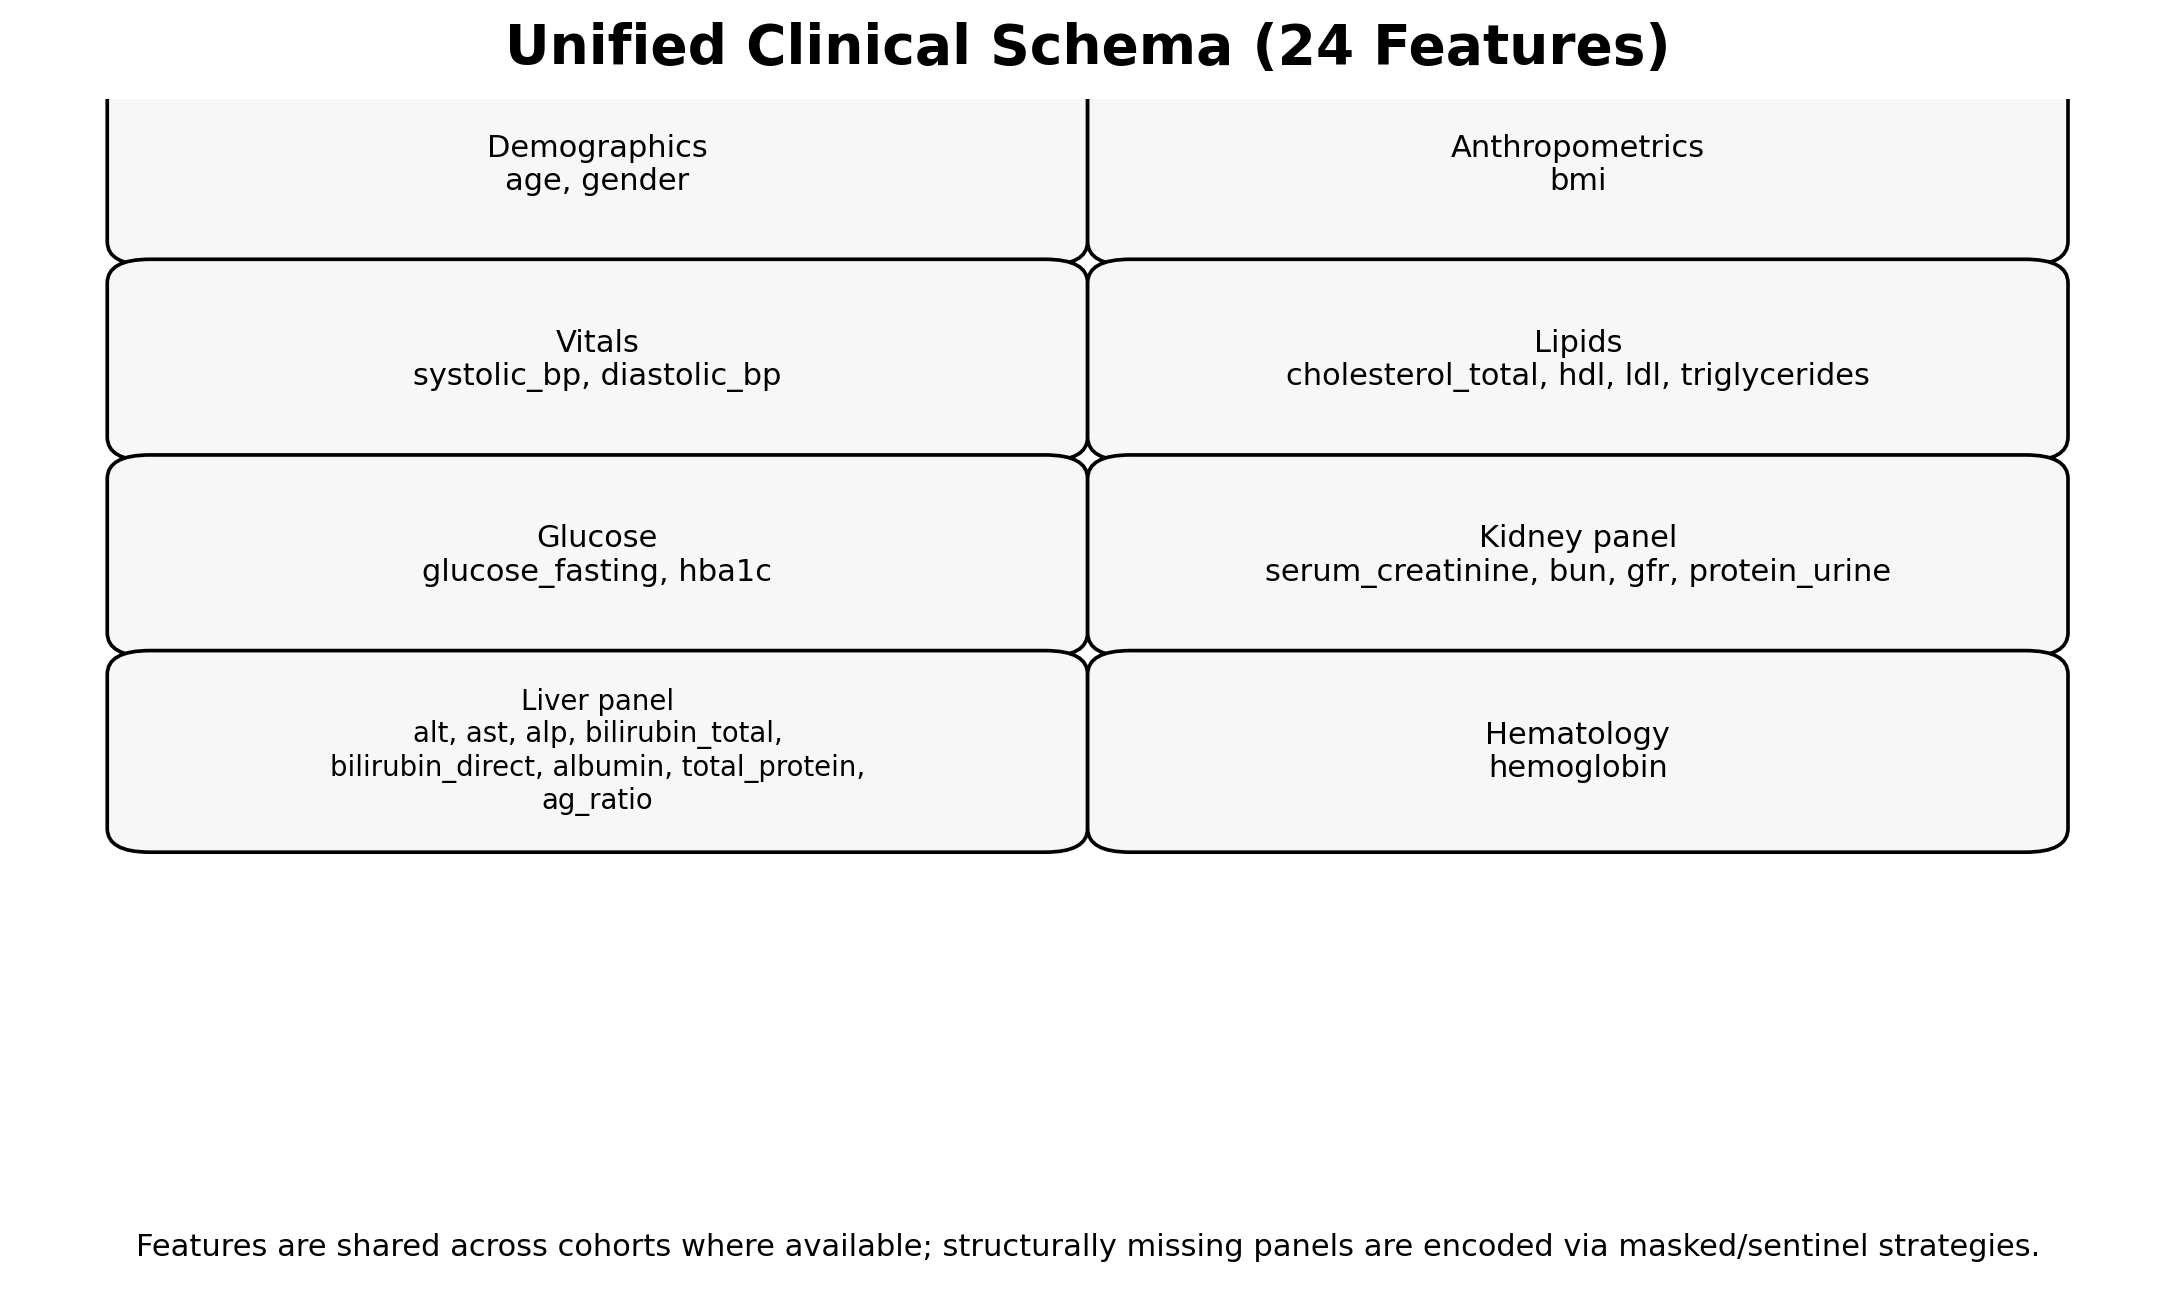
\includegraphics[width=\linewidth]{report_figures/unified_schema_24_features.png}
\caption{Unified clinical schema used across all disease cohorts (24 features grouped by clinical panels).}
\label{fig:schema}
\end{figure}

\section{Structural Missingness and Our Dual-Encoding Strategy}
\subsection{Why Standard Imputation Is Unsafe}
A dominant challenge in multi-disease fusion is \emph{structural missingness}: a biomarker is genuinely unmeasured for an entire cohort because it is not part of that disease panel (e.g., liver enzymes are absent in heart-only records). In such settings, KNN/MICE-style imputers can ``invent'' plausible-looking labs by borrowing from other cohorts, creating medically implausible correlations.

\subsection{Masked Representation (value + mask)}
For deep models (FT-Transformer), we build a masked representation by pairing each feature value $x_j$ with a binary availability indicator $m_j \in \{0,1\}$:
\begin{equation}
\tilde{x}_j = \begin{bmatrix}x_j \\ m_j\end{bmatrix}, \quad m_j=0 \text{ means ``unobserved''}.
\end{equation}
Missing values are imputed with a conservative statistic (median/mode), but the mask ensures the model can learn that an imputed value should be discounted.

\subsection{Sentinel Representation ($-999$)}
For tree-based models, we encode missing numeric values as a single sentinel constant ($-999$). Because standardized real values typically lie near $[-3,3]$, a sentinel far outside this range is easy for decision trees to isolate with split rules.

\begin{figure}[t]
\centering
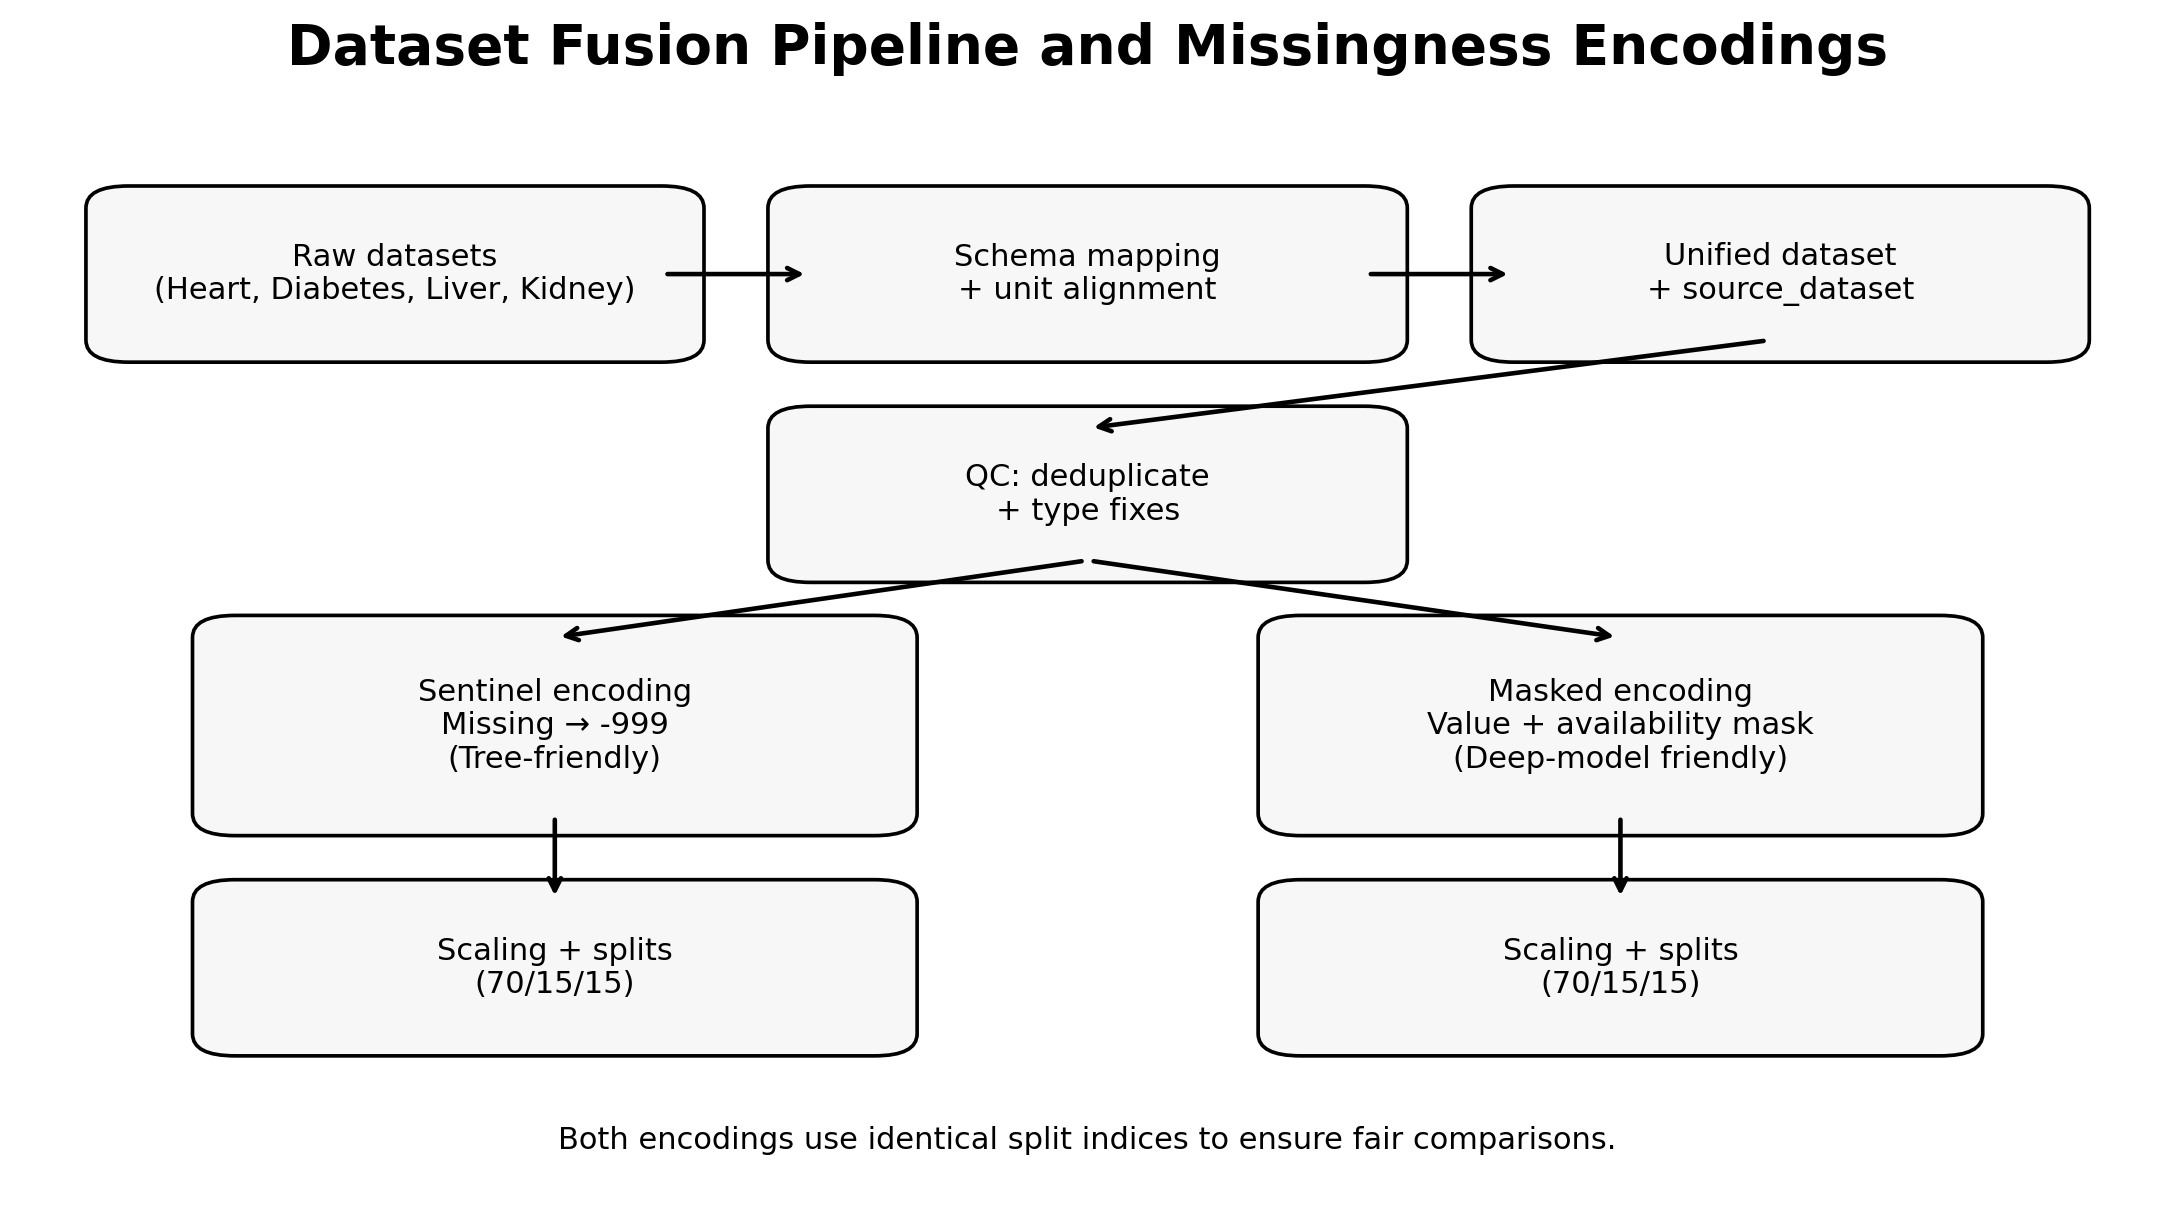
\includegraphics[width=\linewidth]{report_figures/data_pipeline_masked_sentinel.png}
\caption{Dataset fusion pipeline and missingness handling: masked (value+mask) and sentinel ($-999$) encodings.}
\label{fig:missingness}
\end{figure}

\section{Preprocessing and Experimental Protocol}
\subsection{Quality Assurance and Scaling}
We removed exact duplicates (\mbox{\textasciitilde}11,360 rows) and standardized numeric features. For the sentinel version, scaling statistics are computed using only non-sentinel values and the sentinel itself is preserved. For the masked version, only the value columns are scaled while mask columns remain 0/1.

\subsection{Train/Validation/Test Splits}
We create 70/15/15 train/validation/test splits stratified by \texttt{source\_dataset} so each split maintains approximately the same cohort composition. The same indices are applied to both masked and sentinel versions to enable fair comparisons.

\section{Modeling Approaches}
Modeling is the step where we learn a mapping from a patient's structured feature vector to a disease risk score (probability). In our setting, the data is (i) tabular, (ii) clinically heterogeneous across disease cohorts, and (iii) dominated by structural missingness. Therefore, we benchmark multiple model families with complementary strengths: simple linear baselines for interpretability, tree ensembles for non-linear interactions, and a transformer-based deep model to test whether representation learning can outperform boosting on the fused schema.

We treat each disease as a binary classification task. For classical models, we train one model per disease by filtering the unified dataset to rows where that disease label is observed (to avoid treating missing labels as negatives). For the FT-Transformer, we additionally explore a \emph{multi-output} formulation with a masked loss so that a single network can be trained even when only one label is available per row.

For evaluation, we report AUC-ROC as the primary metric because it is threshold-free and more informative than raw accuracy under class imbalance.

\subsection{Classical Machine Learning Baselines: What We Chose and Why}
We selected four widely used baselines that span increasing model capacity and capture different inductive biases for tabular clinical data:
\begin{itemize}
    \item \textbf{Logistic Regression (LR):} a strong, interpretable linear baseline that provides a calibration-friendly reference point.
    \item \textbf{Random Forest (RF):} a bagged tree ensemble that captures non-linear interactions and is robust to noise.
    \item \textbf{XGBoost (XGB):} regularized gradient boosting, a highly competitive choice for structured biomarkers.
    \item \textbf{LightGBM (LGBM):} a histogram-based gradient boosting variant that is often fast and accurate on large tabular datasets.
\end{itemize}

This set is intentionally diverse: it allows a fair comparison between a linear model, a bagging-based ensemble, and two modern boosting implementations. It also reflects practical deployment constraints---these models are lightweight, train quickly, and integrate cleanly into a Python-based application.

\subsubsection{Logistic Regression (LR)}
LR is the simplest baseline and serves two purposes. First, it provides a sanity check that the unified feature mapping contains signal: if LR performs well, the schema and preprocessing are likely consistent. Second, its coefficients (after normalization) provide a coarse, human-readable view of how biomarkers relate to risk. Its limitation is capacity: purely linear decision boundaries cannot represent complex clinical interactions (e.g., age-dependent effects or non-linear thresholds).

\subsubsection{Random Forest (RF)}
RF uses many decision trees trained on bootstrapped samples with feature subsampling. This allows it to represent non-linear relationships and feature interactions without requiring extensive feature engineering. RF is typically robust and stable, but it can be less efficient at fine-grained probability estimation than boosting and may require more trees to achieve the same discrimination performance.

\subsubsection{Gradient Boosting: XGBoost (XGB) and LightGBM (LGBM)}
Gradient boosting builds an additive ensemble of shallow trees, sequentially correcting previous errors while applying regularization. This family is a strong fit for tabular clinical data because it naturally models non-linearities, captures interactions, and is effective even when feature distributions differ across cohorts.

We compare both XGBoost and LightGBM because they represent two high-performing implementations with different engineering trade-offs (split finding, histogram optimizations, regularization defaults). In practice, both are strong candidates for a production demo; our final selection is justified later using the empirical comparison and deployment constraints.

\subsection{Multi-Output FT-Transformer: What It Is and Why We Tried It}
FT-Transformer is a transformer architecture adapted for tabular data. Conceptually, it treats each feature as a learnable token embedding and uses multi-head self-attention to model feature-feature interactions. Compared to tree ensembles, this approach can learn richer representations and potentially share statistical strength across related tasks.

We explored FT-Transformer for two reasons. First, recent literature suggests transformer-style models can be competitive on structured data when trained carefully. Second, our problem has a natural multi-task structure (four diseases) and we hypothesized that a shared backbone could learn reusable ``clinical feature interaction'' patterns across cohorts, potentially outperforming per-disease boosting.

\subsubsection{Handling Structural Missingness in FT-Transformer}
To avoid collapsing ``unobserved'' and ``normal'' values, we use the masked representation described earlier (value + availability indicator). Each input feature is paired with a binary mask that explicitly tells the model whether the biomarker was measured for that cohort. This is important because structural missingness is not random; it encodes how the dataset was collected.

\subsubsection{Multi-Output Training with Masked Loss}
We train a single network with four output heads (one per disease). Let $\hat{y}^{(d)}$ be the predicted probability for disease $d$ and $y^{(d)}$ be the ground-truth label. Because only one disease label is observed for any given row, we define a label-availability mask $m^{(d)} \in \{0,1\}$ and optimize a masked binary cross-entropy:
\begin{equation}
\mathcal{L} = \sum_{d=1}^{4} m^{(d)}\,\mathrm{BCE}(\hat{y}^{(d)}, y^{(d)}).
\end{equation}
This ensures the network learns from each cohort without being penalized for missing labels in the other tasks.

\subsubsection{Configuration Snapshot}
A representative Week~7 configuration uses $d_{token}=64$, 4 transformer layers, 8 attention heads, and dropout regularization (\mbox{\textasciitilde}207k parameters). We compare the resulting model against XGBoost using the stored Week~6 metrics to evaluate whether the increased modeling complexity translates into consistent AUC gains.

\section{Results}
\subsection{ML Baselines (Week 6)}
Table~\ref{tab:week6} summarizes the Week~6 baseline evaluation under sentinel encoding. Tree ensembles consistently outperform LR, and gradient boosting achieves the strongest or near-strongest AUC across tasks.

\begin{table}[t]
\centering
\caption{Week 6 Sentinel Baselines (Test AUC-ROC)}
\label{tab:week6}
\small
\begin{tabular}{lcccc}
\toprule
\textbf{Disease} & \textbf{LR} & \textbf{RF} & \textbf{XGB} & \textbf{LGBM} \\
\midrule
Heart   & 0.7864 & 0.7927 & 0.7905 & \textbf{0.7935} \\
Diabetes& 0.9331 & \textbf{0.9414} & 0.9413 & 0.9406 \\
Liver   & 0.5133 & 0.9991 & \textbf{0.9992} & 0.9991 \\
Kidney  & 0.8490 & 0.9288 & \textbf{0.9362} & 0.9322 \\
\bottomrule
\end{tabular}
\end{table}

\subsection{FT-Transformer vs. XGBoost (Comparison.md Evidence)}
For the report-required head-to-head comparison, we cite the stored Week~6 sentinel comparison between XGBoost and FT-Transformer (from \texttt{comparison.md}). FT-Transformer slightly improves heart AUC, while XGBoost is higher on diabetes, liver, and kidney.

\begin{figure}[t]
\centering
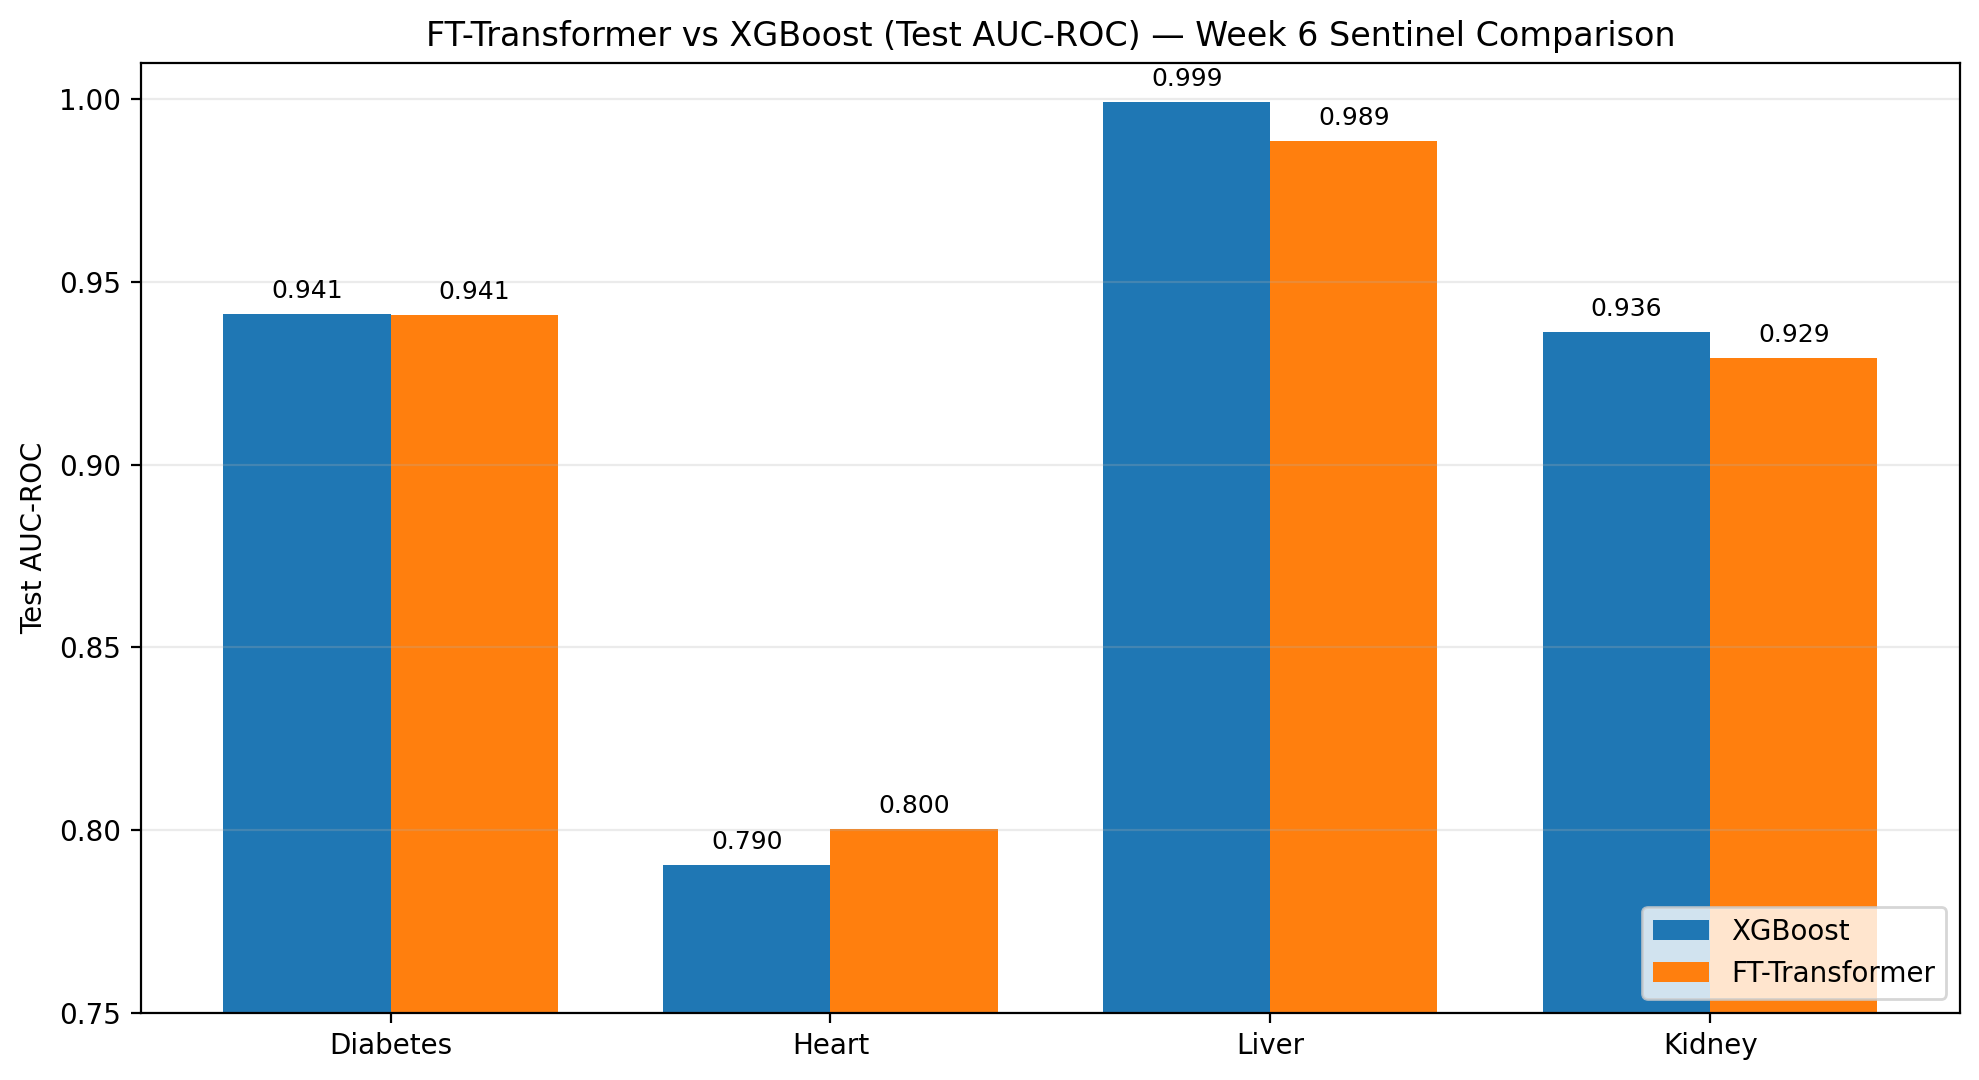
\includegraphics[width=\linewidth]{report_figures/auc_ft_vs_xgb_week6.png}
\caption{FT-Transformer vs. XGBoost test AUC-ROC (Week 6 sentinel comparison).}
\label{fig:ftxgb}
\end{figure}

\begin{table}[t]
\centering
\caption{FT-Transformer vs. XGBoost (Week 6 Sentinel Comparison)}
\label{tab:ftxgb}
\small
\begin{tabular}{lccc}
\toprule
\textbf{Disease} & \textbf{XGBoost} & \textbf{FT-Transformer} & $\boldsymbol{\Delta}$ \\
\midrule
Diabetes & 0.9413 & 0.9410 & $-0.0003$ \\
Heart    & 0.7905 & 0.8002 & $+0.0097$ \\
Liver    & 0.9992 & 0.9886 & $-0.0106$ \\
Kidney   & 0.9362 & 0.9292 & $-0.0070$ \\
\bottomrule
\end{tabular}
\end{table}

\subsection{Why We Deployed XGBoost}
Model selection for the deployed Semester~1 demo is not driven by AUC alone. We also require a model that is fast at inference, easy to version and load, robust under structural missingness, and compatible with faithful feature attribution in the UI. Across our baseline comparisons, gradient boosting models (XGBoost/LightGBM) are consistently strong on tabular biomarkers, while the FT-Transformer shows mixed gains (an improvement on heart, but lower AUC on the other three tasks in the Week~6 comparison).

In Table~\ref{tab:week6}, LightGBM is marginally higher on heart and Random Forest is marginally higher on diabetes, but XGBoost remains consistently near-best across all four diseases. This ``strong across tasks'' behavior is valuable for an end-to-end system because it lets us standardize training, persistence, and explanation workflows across diseases.

Even when FT-Transformer is competitive, we selected XGBoost for deployment because it provides the best overall balance of (i) discrimination performance across diseases, (ii) engineering simplicity, and (iii) explainability support:
\begin{enumerate}
    \item \textbf{Consistently strong discrimination:} in the required Week~6 comparison, XGBoost is higher on 3/4 diseases. While the differences are not always large, the overall pattern indicates that boosting remains a reliable choice for our fused tabular schema.
    \item \textbf{Operational simplicity for an end-to-end demo:} XGBoost models are lightweight, fast at inference, and straightforward to persist and reload (e.g., via \texttt{.pkl}/joblib), which reduces friction when integrating with Streamlit.
    \item \textbf{Explainability readiness:} TreeSHAP provides efficient, additive feature attributions aligned with the model's structure, enabling reliable local (per-patient) and global explanations without introducing a separate surrogate model.
\end{enumerate}

\section{Explainable AI Integration (SHAP)}
We integrate SHAP explanations into the Streamlit frontend to answer the core requirement: \emph{which features drive the risk score?} For each disease prediction, we compute per-patient attributions and surface the top increasing/decreasing factors with clinical context (raw value and normal-range status). We also compute global feature importance using a bounded reference sample to keep the app responsive.

\begin{figure}[t]
\centering
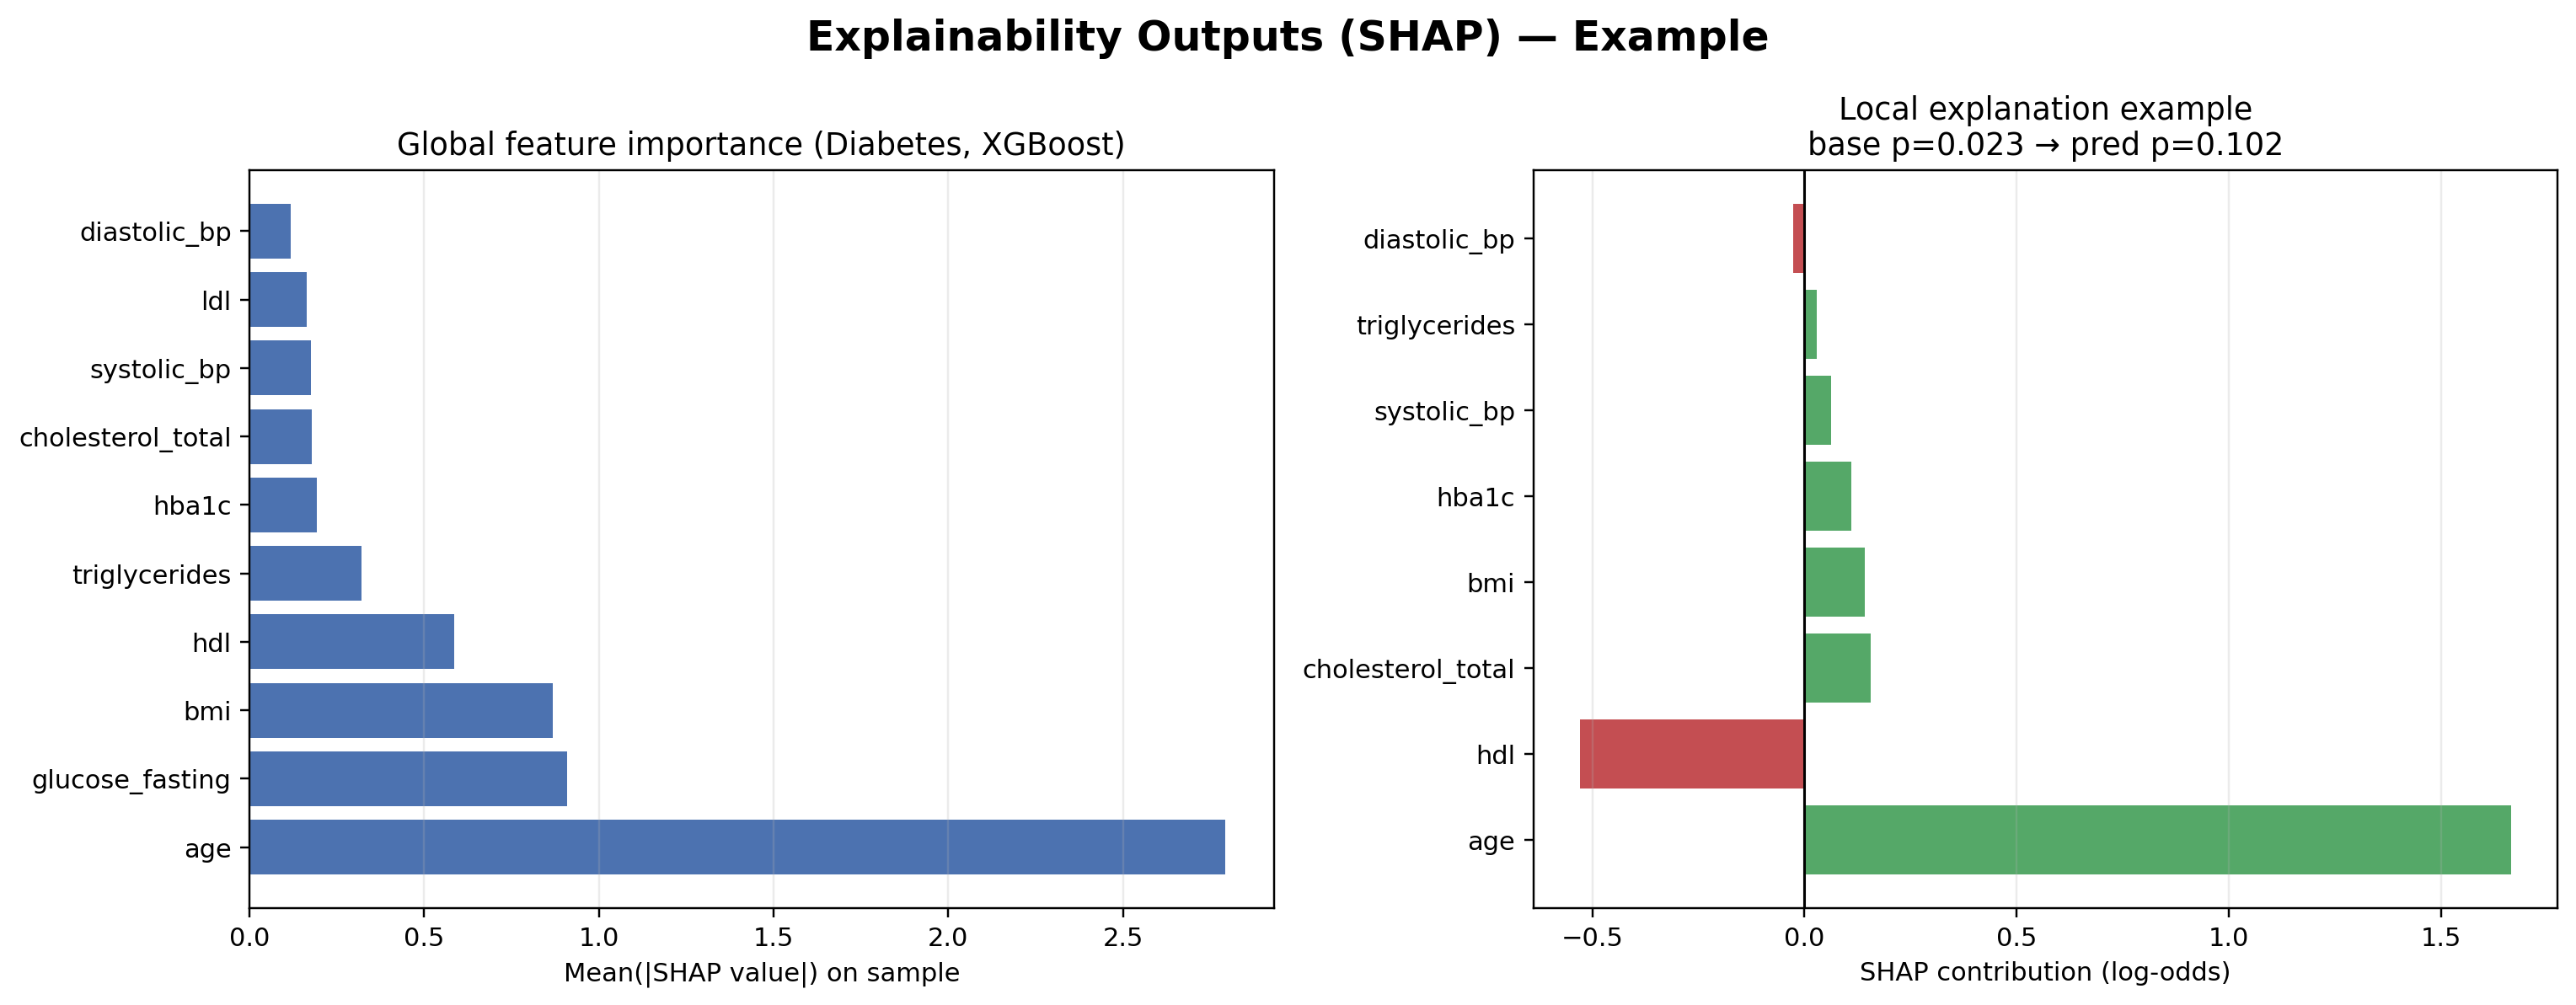
\includegraphics[width=\linewidth]{report_figures/shap_explainability_ui.png}
\caption{Example SHAP outputs for the deployed XGBoost model: global feature importance (mean absolute SHAP) and a local per-patient explanation (log-odds contributions).}
\label{fig:shap}
\end{figure}

\section{Application and Deployment}
\subsection{Streamlit Frontend}
The interactive application is implemented in \texttt{webapp/app.py}. It supports per-patient prediction for all four diseases, SHAP-based explainability panels, and an ``AI Explanation \& Chat'' section.

\begin{figure}[t]
\centering
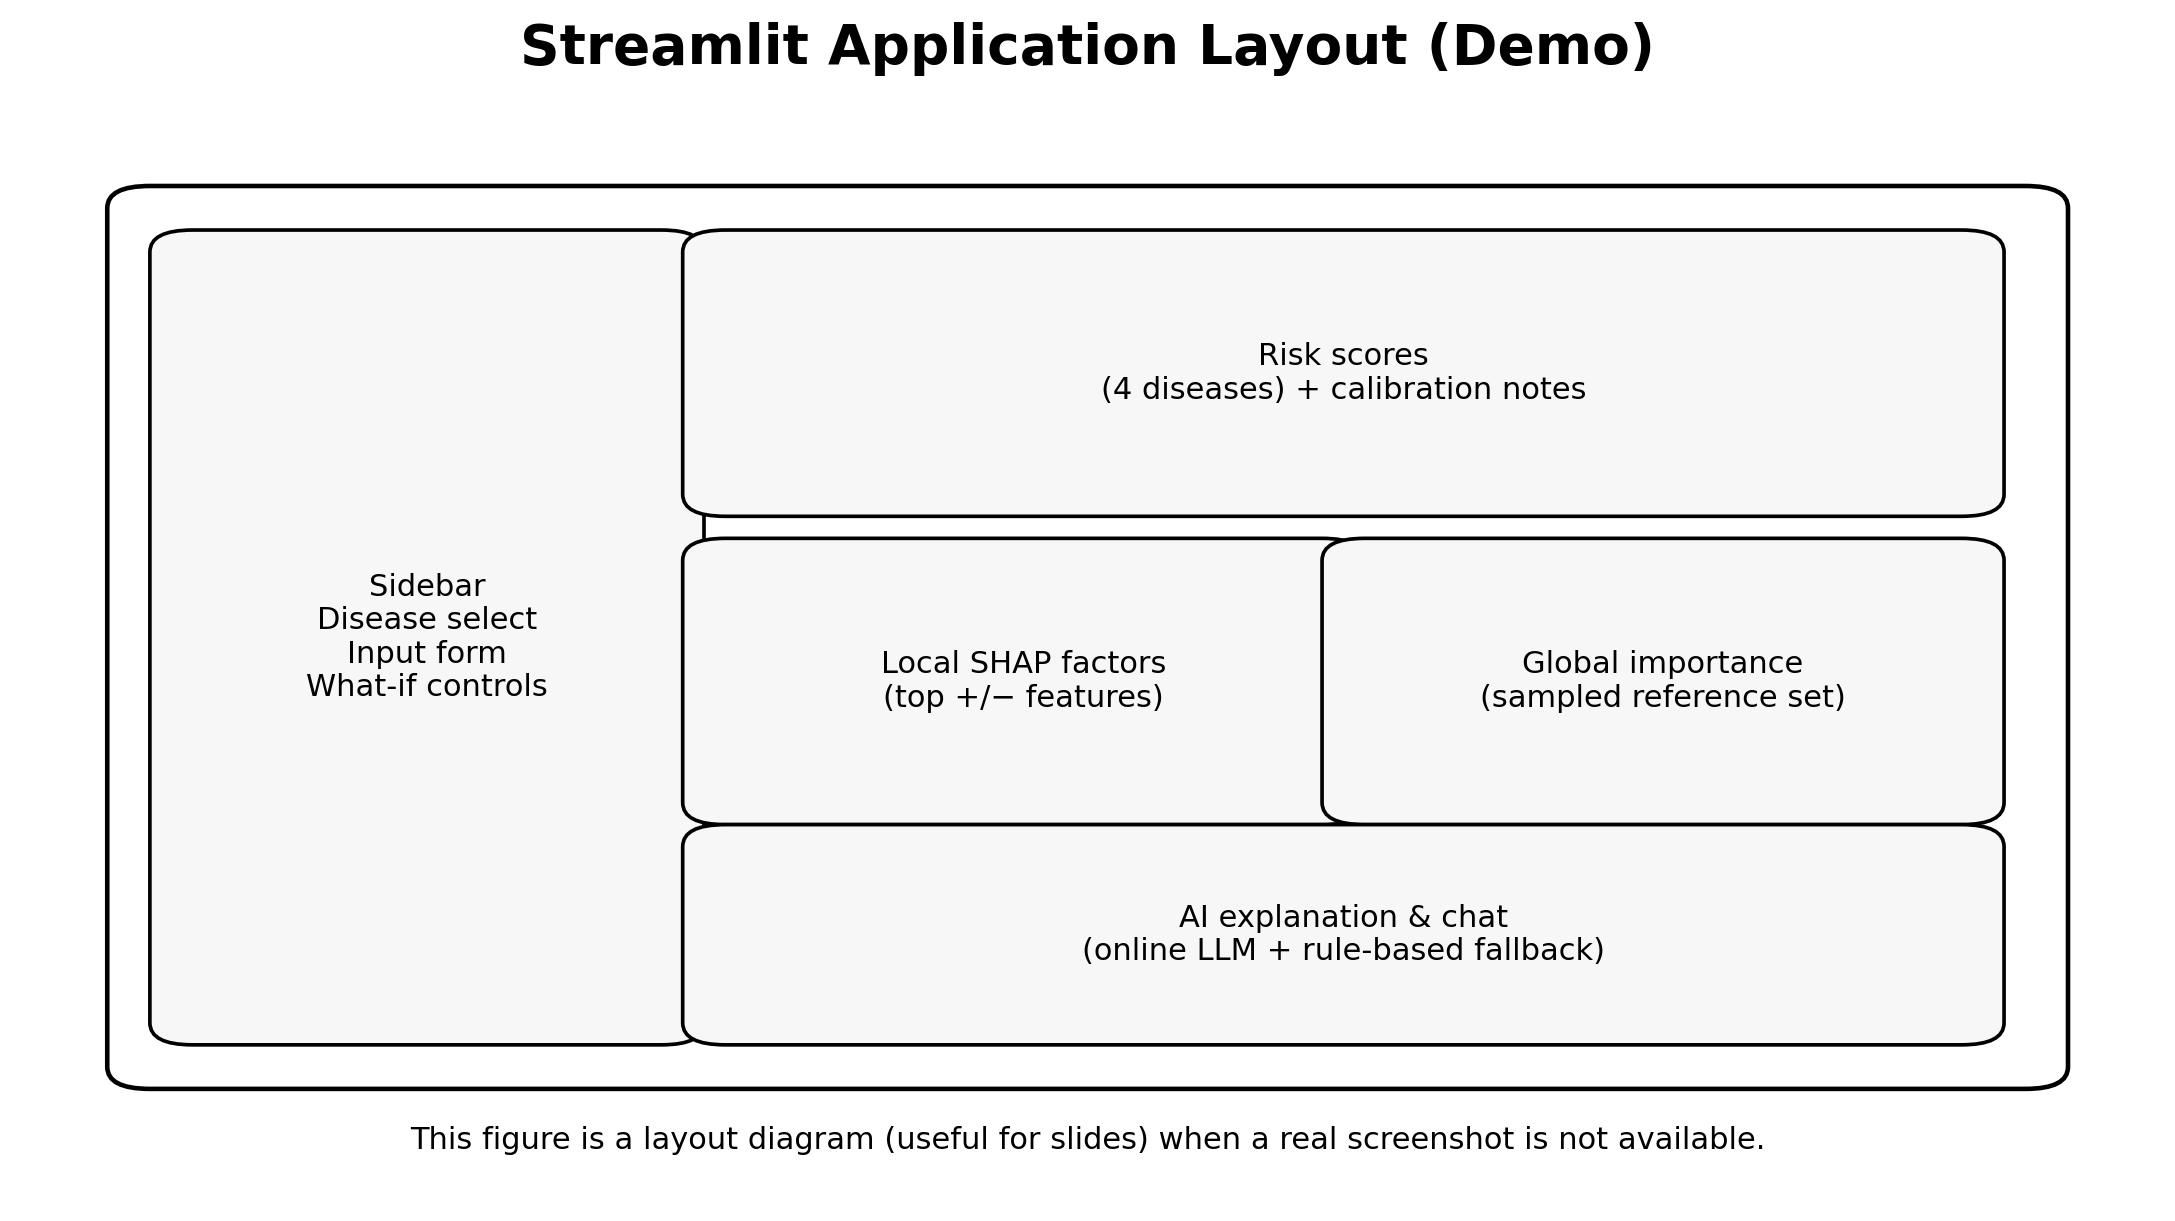
\includegraphics[width=\linewidth]{report_figures/streamlit_app_screenshot.png}
\caption{Streamlit application layout showing risk scores, SHAP explainability panels, and the AI chat section.}
\label{fig:ui}
\end{figure}

\subsection{Online LLM Integration (Provider-Agnostic)}
To avoid local model downloads and support constrained storage environments, we integrated an OpenAI-compatible HTTP client that can target providers such as Groq or OpenAI using environment variables (e.g., \texttt{BTP\_LLM\_BASE\_URL}, \texttt{BTP\_LLM\_API\_KEY}, \texttt{BTP\_LLM\_MODEL}). The LLM receives a compact JSON payload containing the predicted risk, structured SHAP factors, and rule-based disease guidance. Safety constraints are enforced: the assistant provides health education, not diagnosis; it does not prescribe or give dosing; it may mention medication \emph{classes} only as clinician discussion topics.

\begin{figure}[t]
\centering
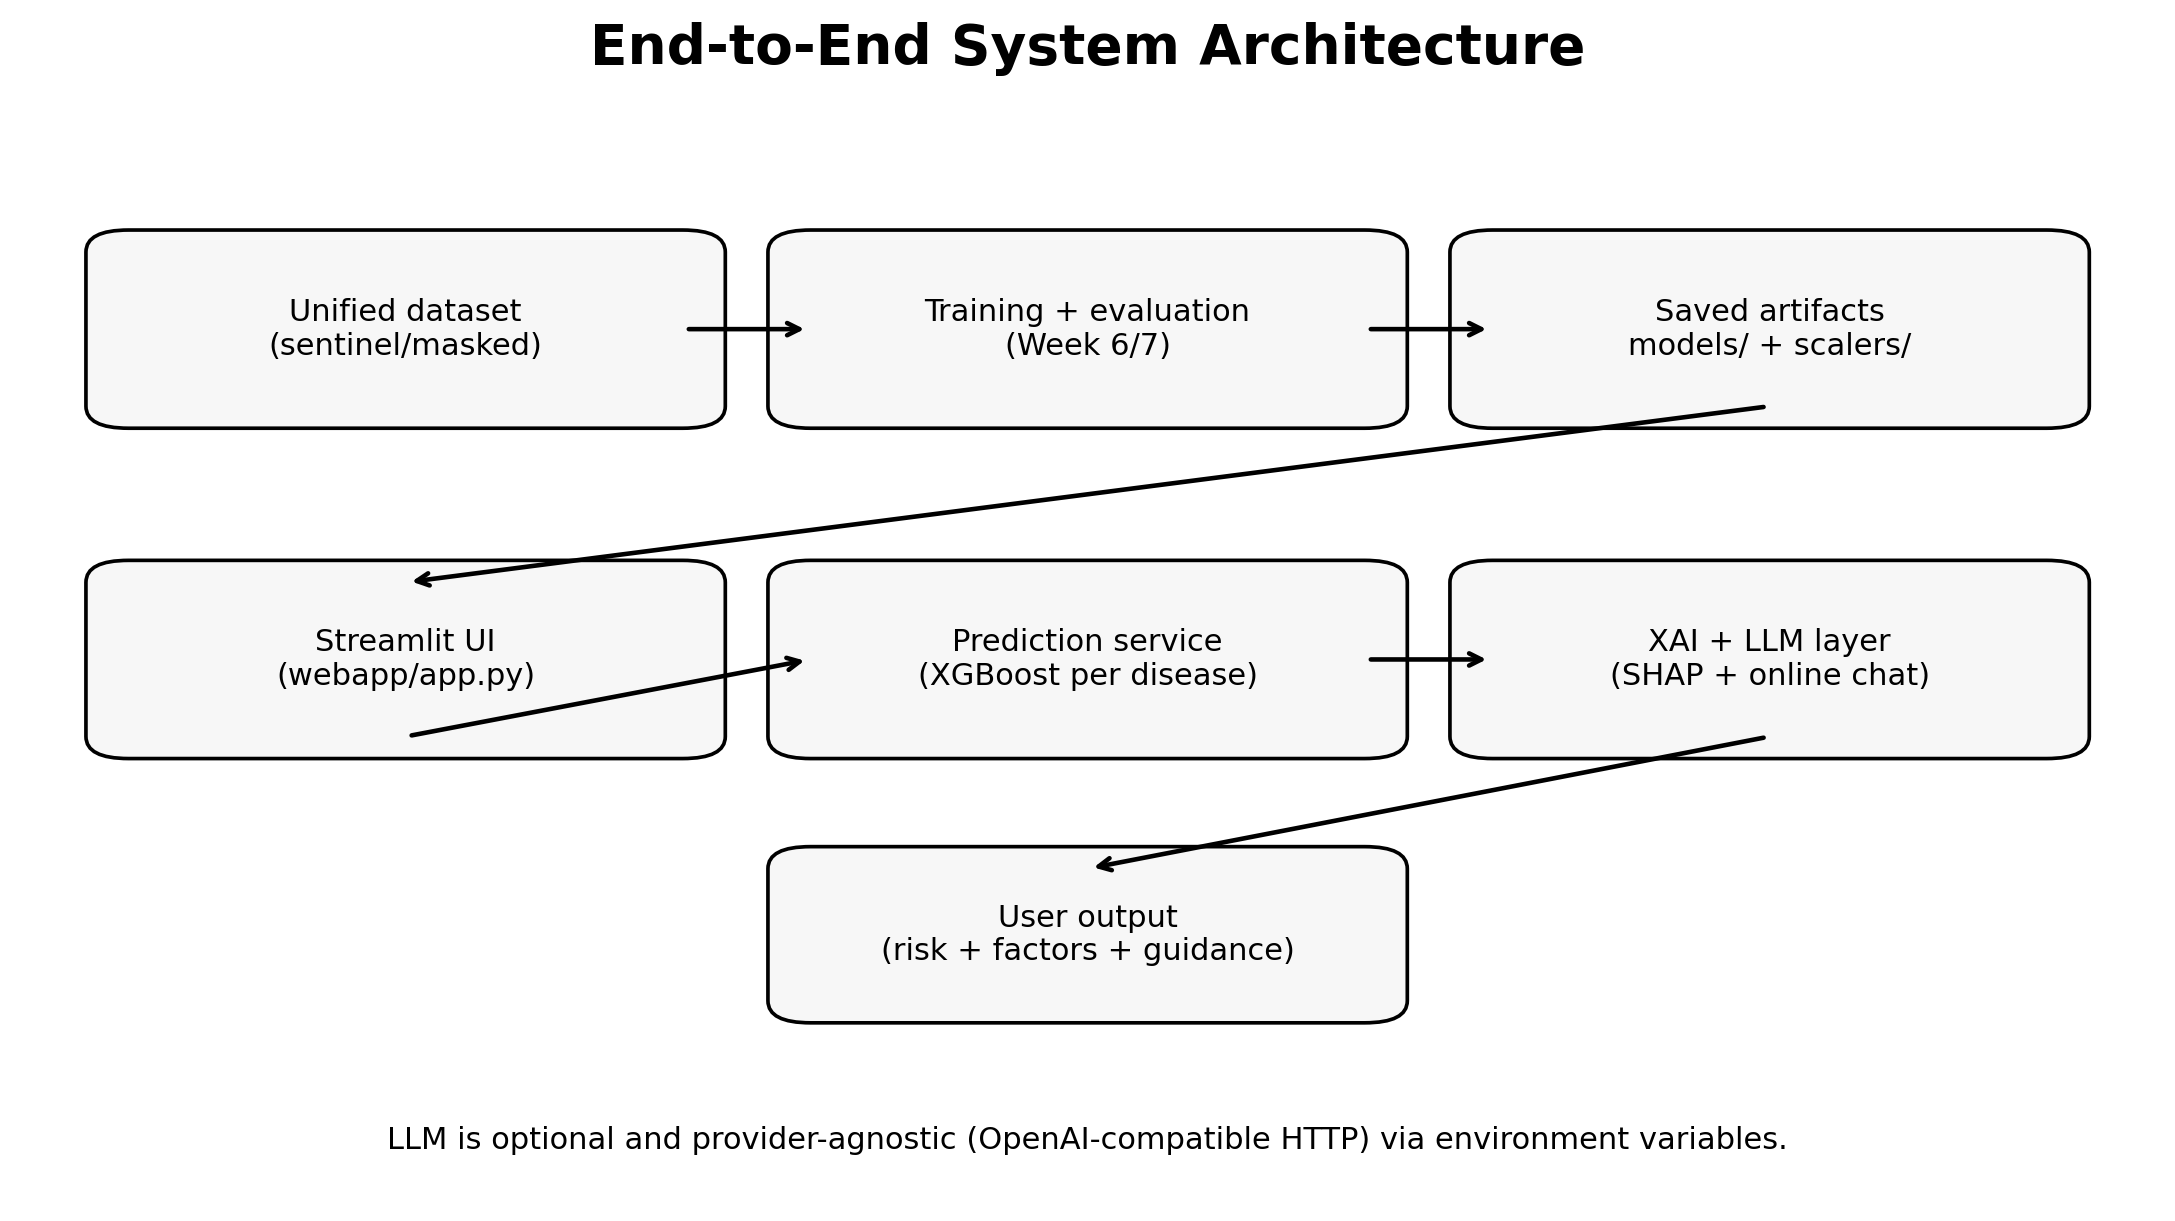
\includegraphics[width=\linewidth]{report_figures/system_architecture.png}
\caption{End-to-end system architecture from unified dataset and trained artifacts to Streamlit inference, SHAP explainability, and optional online LLM guidance.}
\label{fig:arch}
\end{figure}

\section{Discussion and Limitations}
Our primary scientific contribution is a missingness-aware fusion strategy aligned with clinical measurement realities. Limitations include: (i) dataset heterogeneity and differing label definitions across sources, (ii) the need for stronger calibration and external validation on clinical cohorts, and (iii) preprocessing choices (e.g., scaling on aggregated data) that should be tightened for production-grade evaluation.

\section{Future Work (Semester 2)}
Planned extensions include: integrating unstructured clinical text (clinical notes, patient histories) via medical NLP; expanding capture of lifestyle habits; improving calibration and uncertainty estimation; completing the end-to-end application with production-grade FastAPI prediction and explainability routes; exploring agentic AI workflows for automated report writing from experiment logs; and expanding evaluation to multi-site datasets with stronger generalization testing.

\section{Conclusion}
We delivered an end-to-end multi-disease risk prediction prototype that fuses heterogeneous tabular datasets into a unified schema, addresses structural missingness via masked and sentinel encodings, and provides a usable Streamlit application with SHAP-based explainability and an online LLM-powered guidance layer. Empirically, gradient boosting remains a strong choice for tabular clinical biomarkers, and XGBoost provides an effective balance of accuracy, deployability, and explainability for the current demo.

\begin{thebibliography}{99}
\bibitem{chen2016xgboost}
T.~Chen and C.~Guestrin, ``XGBoost: A scalable tree boosting system,'' in \emph{Proc. ACM SIGKDD}, 2016.

\bibitem{ke2017lightgbm}
G.~Ke \emph{et al.}, ``LightGBM: A highly efficient gradient boosting decision tree,'' in \emph{Proc. NeurIPS}, 2017.

\bibitem{lundberg2017shap}
S.~M. Lundberg and S.-I. Lee, ``A unified approach to interpreting model predictions,'' in \emph{Proc. NeurIPS}, 2017.

\bibitem{gorishniy2021revisiting}
Y.~Gorishniy, I.~Rubachev, V.~Khrapov, and A.~Babenko, ``Revisiting deep learning models for tabular data,'' in \emph{Proc. NeurIPS}, 2021.

\bibitem{johnson2016mimic}
A.~E. W. Johnson \emph{et al.}, ``MIMIC-III, a freely accessible critical care database,'' \emph{Scientific Data}, 2016.
\end{thebibliography}

\end{document}
